\chapter{Introducción}

En este trabajo nos centraremos en el control y coordinación de varios UAVs, principalmente en la subcategoría conocida como cuadricópteros, popularmente llamados drones. 

Se propone como objetivo final conseguir la coordinación entre \textit{Crazyflies}, cuadricópteros ligeros desarrollados por la empresa Bitcraze,
mediante la implementación de un firmware de código abierto basado en el proyecto \textit{Paparazzi UAV} 
\cite{paparazzi_github} y la inclusión de un algoritmo para coordinación.

%%%%%%%%%%%%%%%%%%%%%%%%%%%%%%%%%%%%%%%%%%%%%%%%%%%%%%%%%%%%%%%%%%%%%%%%%%%%%%%%%%%%%%%%%%%%%%%%%%%%%%%%%%%%%%%%%
%%%%%%%%%%%%%%%%%%%%%%%%%%%%%%%%%%%%%%%%%%%%%%%%%%%%%%%%%%%%%%%%%%%%%%%%%%%%%%%%%%%%%%%%%%%%%%%%%%%%%%%%%%%%%%%%%
%%%%%%%%%%%%%%%%%%%%%%%%%%%%%%%%%%%%%%%%%%%%%%%%%%%%%%%%%%%%%%%%%%%%%%%%%%%%%%%%%%%%%%%%%%%%%%%%%%%%%%%%%%%%%%%%%

\section{Motivación}

Los drones Crazyflie son una plataforma ideal para explorar conceptos de control, comunicación y coordinación en robótica. 
Este TFG permitirá desarrollar habilidades prácticas en programación, electrónica y sistemas embebidos, 
así como aplicar teorías complejas de control y algoritmos de coordinación en un entorno real y simulado paralelamente.

Los drones tienen numerosas aplicaciones prácticas, desde la vigilancia y el rescate hasta la agricultura de precisión o entrega de mercancías. 
Desafortunadamente, existen limitaciones tanto hardware como software en el mundo de la robótica, por ejemplo,
las limitaciones de batería o el simple control por \textit{waypoints} de un dron.

Muchas de estas limitaciones se pueden sobrepasar aplicando enjambres de drones, permitiendo que las aplicaciones
prácticas actuales puedan expandirse e incluso permitir nuevas aplicaciones que previamente
eran impensables con el control limitado de un sólo dron.

En general, este TFG tiene como objetivo el avance en el control y, en especial, coordinación entre sistemas
de dos o más robots, aplicados al entorno de los drones.

%%%%%%%%%%%%%%%%%%%%%%%%%%%%%%%%%%%%%%%%%%%%%%%%%%%%%%%%%%%%%%%%%%%%%%%%%%%%%%%%%%%%%%%%%%%%%%%%%%%%%%%%%%%%%%%%%
%%%%%%%%%%%%%%%%%%%%%%%%%%%%%%%%%%%%%%%%%%%%%%%%%%%%%%%%%%%%%%%%%%%%%%%%%%%%%%%%%%%%%%%%%%%%%%%%%%%%%%%%%%%%%%%%%
%%%%%%%%%%%%%%%%%%%%%%%%%%%%%%%%%%%%%%%%%%%%%%%%%%%%%%%%%%%%%%%%%%%%%%%%%%%%%%%%%%%%%%%%%%%%%%%%%%%%%%%%%%%%%%%%%

\section{Descripción general del sistema}

Para la coordinación entre dispositivos necesitaremos como mínimo dos o más Crazyflies, 
un accesorio para localización como, por ejemplo, el de Bitcraze por \textit{anchors} para los Crazyflies 
y un dispositivo de control central, generalmente un portátil con un software para el control de los UAVs.

Los términos \textbf{UAV, rotorcraft y dron} se utilizarán indistintamente para referirnos, por lo general, 
a los Crazyflies u otro dispositivo similar.

En las siguientes subsecciones detallaremos cada componente del sistema individualmente, divididos por hardware y software.

%%%%%%%%%%%%%%%%%%%%%%%%%%%%%%%%%%%%%%%%%%%%%%%%%%%%%%%%%%%%%%%%%%%%%%%%%%%%%%%%%%%%%%%%%%%%%%%%%%%%%%%%%%%%%%%%%
%%%%%%%%%%%%%%%%%%%%%%%%%%%%%%%%%%%%%%%%%%%%%%%%%%%%%%%%%%%%%%%%%%%%%%%%%%%%%%%%%%%%%%%%%%%%%%%%%%%%%%%%%%%%%%%%%
%%%%%%%%%%%%%%%%%%%%%%%%%%%%%%%%%%%%%%%%%%%%%%%%%%%%%%%%%%%%%%%%%%%%%%%%%%%%%%%%%%%%%%%%%%%%%%%%%%%%%%%%%%%%%%%%%

\subsection{Hardware: Crazyflies y accesorios}

Se trabajará concretamente con los \textbf{Crazyflie 2.1}, drones de tan solo 27 gramos y dimensiones 92x92x29mm \cite{crazyflie_product_page}.
Su bajo peso y tamaño implican que tan solo es deseable usarlos en espacios interiores.
Entre sus características más destacables, se encuentra la capacidad de sustituir el firmware oficial, consecuencia de ser un dispositivo 
\textit{open source} y lo que nos permitirá que este trabajo pueda llevarse a cabo.

\begin{figure}[h]
    \centering
    % Crop left, bottom, right, top
    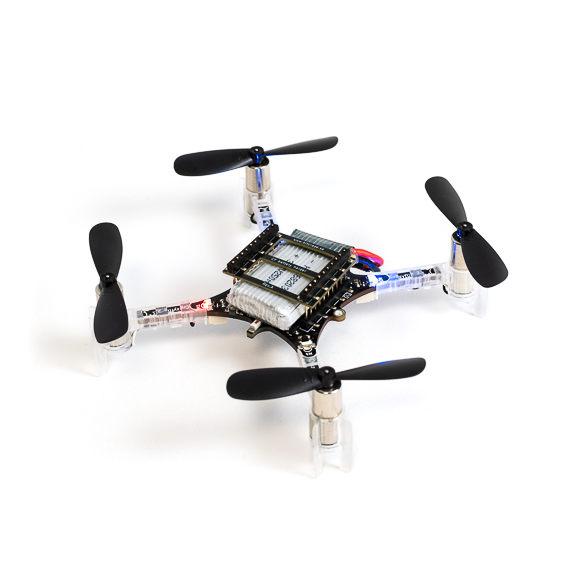
\includegraphics[trim={0 8mm 0 8mm}, clip, width=0.7\textwidth]{img/fig/fig1.1-crayzflie.jpg}
    \caption{Imagen de un Crazyflie 2.1 montado}
    \label{fig:crazyflie}
\end{figure}

Aunque los Crazyflies se pueden utilizar independientemente con un mando radiocontrol o un portátil con el conjunto del software y firmware oficial, 
el objetivo es la coordinación de movimientos entre los drones, por tanto necesitamos conocer la posición relativa o absoluta de todos los drones en tiempo real.
Por ejemplo, Bitcraze dispone de unos módulos basados en UWB (\textit{Ultra WideBand}, banda ultraancha en español) que permiten la localización de los Crazyflies en el espacio con buena precisión.
Este sistema, llamado \textit{\textbf{Loco Positioning System}} se divide en dos componentes \cite{loco_positioning_system}:

\begin{itemize}
  \item \textbf{Loco Positioning Node:} conocidos como \textit{anchors} al estar estáticos en una sala como puntos de referencia. 
  Se sitúan al menos 6 para permitir la triangulización en tres dimensiones de la posición de un Crazyflie.
  Utilizan los módulos de UWB Decawave DWM1000, ampliamente usados y conocidos módulos de UWB.
  
  \item \textbf{Loco Positioning Deck:} módulo de expansión para un Crazyflie, que le permite comunicarse con las \textit{anchors}. También utiliza los Decawave DWM1000.
\end{itemize}

\begin{figure}[h]
    \centering
    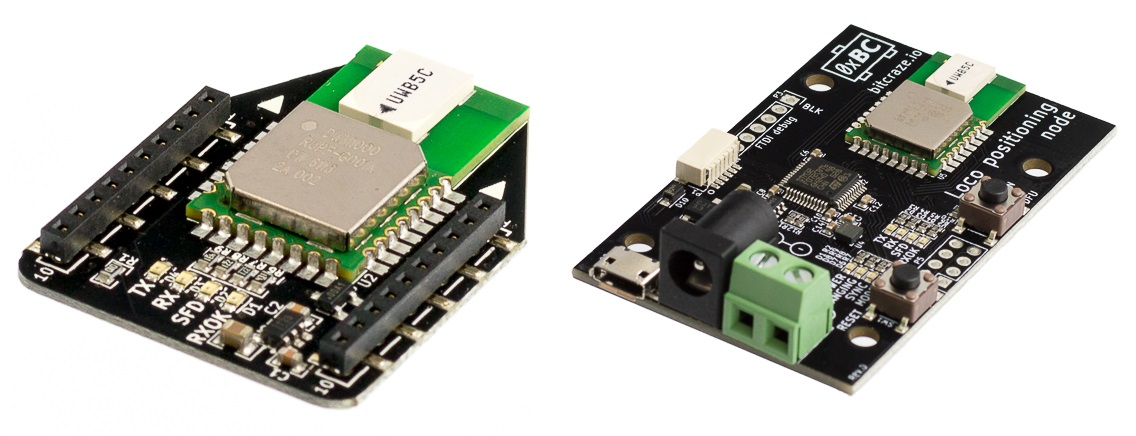
\includegraphics[clip, width=0.7\textwidth]{img/fig/fig1.2-loco-positioning-system.jpg}
    \caption{Loco Positioning Deck (izquierda). Loco Positioning Node (derecha)}
    \label{fig:loco_positioning_system}
\end{figure}

Alternativamente, tenemos otro tipo de accesorio simplificado que, 
si bien tiene menos precisión, es menos dependiente de infraestructura externa.
Se detallará en el capítulo 3, al no cobrar sentido su uso hasta ese capítulo.

%%%%%%%%%%%%%%%%%%%%%%%%%%%%%%%%%%%%%%%%%%%%%%%%%%%%%%%%%%%%%%%%%%%%%%%%%%%%%%%%%%%%%%%%%%%%%%%%%%%%%%%%%%%%%%%%%
%%%%%%%%%%%%%%%%%%%%%%%%%%%%%%%%%%%%%%%%%%%%%%%%%%%%%%%%%%%%%%%%%%%%%%%%%%%%%%%%%%%%%%%%%%%%%%%%%%%%%%%%%%%%%%%%%
%%%%%%%%%%%%%%%%%%%%%%%%%%%%%%%%%%%%%%%%%%%%%%%%%%%%%%%%%%%%%%%%%%%%%%%%%%%%%%%%%%%%%%%%%%%%%%%%%%%%%%%%%%%%%%%%%

\subsection{Software: Paparazzi UAV}

Las pruebas iniciales con el sistema serán con el conjunto del firmware oficial para los Crazyflies y el software oficial para ordenador. 
Una vez se verifique el correcto funcionamiento de cada dron, se pasará al firmware de Paparazzi para los Crazyflies. 
Junto al software de control, \textbf{Paparazzi Center} y \textbf{Paparazzi Ground Control Station} \cite{paparazzi_gcs} se completa la configuración e instalación del sistema para el control y coordinación de los UAV.

\begin{figure}[h]
    \centering
    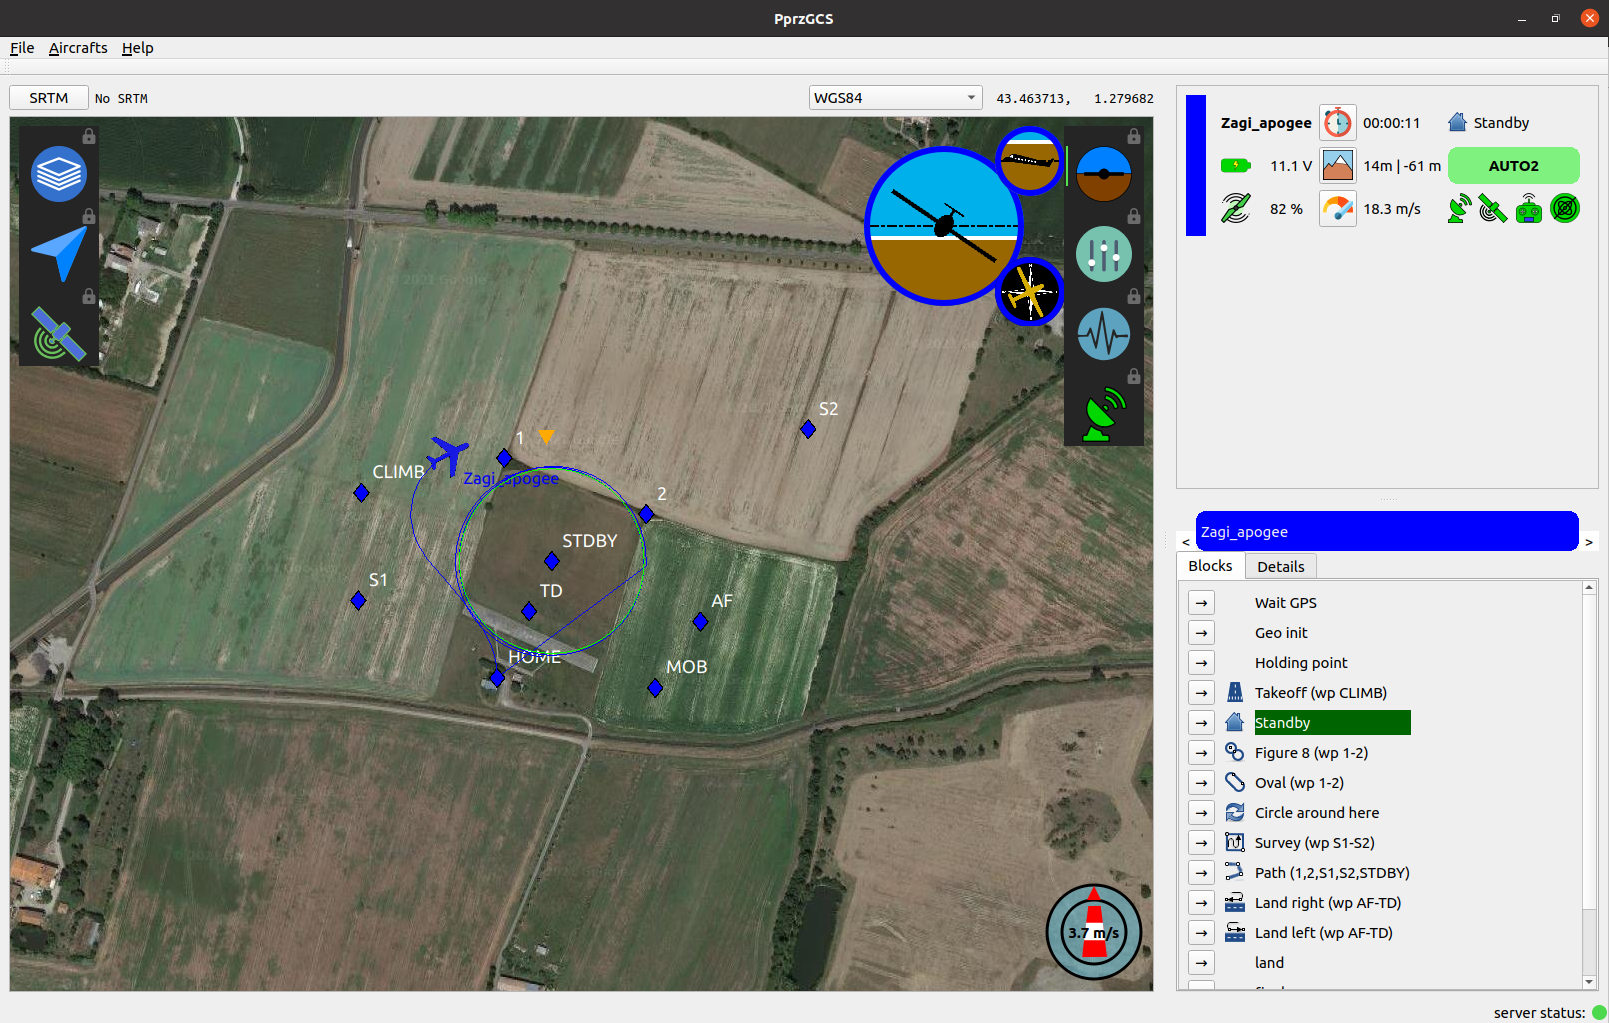
\includegraphics[width=0.88\textwidth]{img/fig/fig1.3-paparazzi-gcs.png}
    \caption{Captura de la interfaz de Paparazzi GCS}
    \label{fig:paparazzi_gcs}
\end{figure}

Para conseguir un funcionamiento completo del sistema, se necesita la implementación del posicionamiento en Paparazzi. 
Actualmente solo se dispone del firmware para los Crazyflie \cite{paparazzi_crazyflie} 
el cual únicamente permite un funcionamiento básico sin posicionamiento preciso,
al depender de exclusivamente los valores del acelerómetro.

%%%%%%%%%%%%%%%%%%%%%%%%%%%%%%%%%%%%%%%%%%%%%%%%%%%%%%%%%%%%%%%%%%%%%%%%%%%%%%%%%%%%%%%%%%%%%%%%%%%%%%%%%%%%%%%%%
%%%%%%%%%%%%%%%%%%%%%%%%%%%%%%%%%%%%%%%%%%%%%%%%%%%%%%%%%%%%%%%%%%%%%%%%%%%%%%%%%%%%%%%%%%%%%%%%%%%%%%%%%%%%%%%%%
%%%%%%%%%%%%%%%%%%%%%%%%%%%%%%%%%%%%%%%%%%%%%%%%%%%%%%%%%%%%%%%%%%%%%%%%%%%%%%%%%%%%%%%%%%%%%%%%%%%%%%%%%%%%%%%%%

\section{Objetivos}

Dada la descripción general del sistema, ya es posible entender los objetivos de este trabajo de fin de grado. Los objetivos, ordenados por capítulos y en orden cronológico de desarrollo, son los siguientes:

\begin{itemize}
    \item \textbf{OBJ-1:} introducción, objetivos, planificación y preparación general. 
    Preparación para la realización de este TFG, incluyendo la realización de este capítulo, familiarización con el ámbito, preparar la plantilla de LaTeX...
    
    \item \textbf{Capítulo 2 (OBJ-2):} preliminares. 
    Se trata de verificar que el hardware funciona de forma correcta siguiendo los pasos del fabricante, así como una breve familiarización con el control básico de un rotorcraft. 
    Tras verificación con el firmware y software oficial, se realizarán las mismas pruebas básicas con Paparazzi.

    \item \textbf{Capítulo 3 (OBJ-3):} control de un Crazyflie. 
    Se conseguirá un control mínimo y estabilizado de un solo Crazyflie (\textit{hovering}).
    Se usará un algoritmo de seguimiento de trayectorias que será implementado en el firmware de Paparazzi.

    \item \textbf{Capítulo 4 (OBJ-4):} coordinación entre Crazyflies. 
    Se añade al objetivo 3 la capacidad de coordinar dos o más drones para seguir trayectorias de forma coordinada (formaciones).

    \item \textbf{Capítulo 5 (OBJ-5):} terminamos este TFG con las conclusiones extraídas, resultados obtenidos, análisis de la planificación y objetivos cumplidos.

    \item \textbf{OBJ-6:} Revisión y mejora general previo de este trabajo. Afecta a todos los objetivos.
    Se añade la realización completa de la presentación en diapositivas y la finalización de esta memoria.
\end{itemize}

Resumidamente, se trata de conseguir que los Crazyflies puedan seguir trayectorias de forma coordinada utilizando el conjunto de firmware y software \textit{open source} de Paparazzi UAV.

%%%%%%%%%%%%%%%%%%%%%%%%%%%%%%%%%%%%%%%%%%%%%%%%%%%%%%%%%%%%%%%%%%%%%%%%%%%%%%%%%%%%%%%%%%%%%%%%%%%%%%%%%%%%%%%%%
%%%%%%%%%%%%%%%%%%%%%%%%%%%%%%%%%%%%%%%%%%%%%%%%%%%%%%%%%%%%%%%%%%%%%%%%%%%%%%%%%%%%%%%%%%%%%%%%%%%%%%%%%%%%%%%%%
%%%%%%%%%%%%%%%%%%%%%%%%%%%%%%%%%%%%%%%%%%%%%%%%%%%%%%%%%%%%%%%%%%%%%%%%%%%%%%%%%%%%%%%%%%%%%%%%%%%%%%%%%%%%%%%%%

\section{Planificación}

Para cumplir los objetivos provistos se ha realizado la siguiente planificación:

\begin{figure}[h]
    \centering
    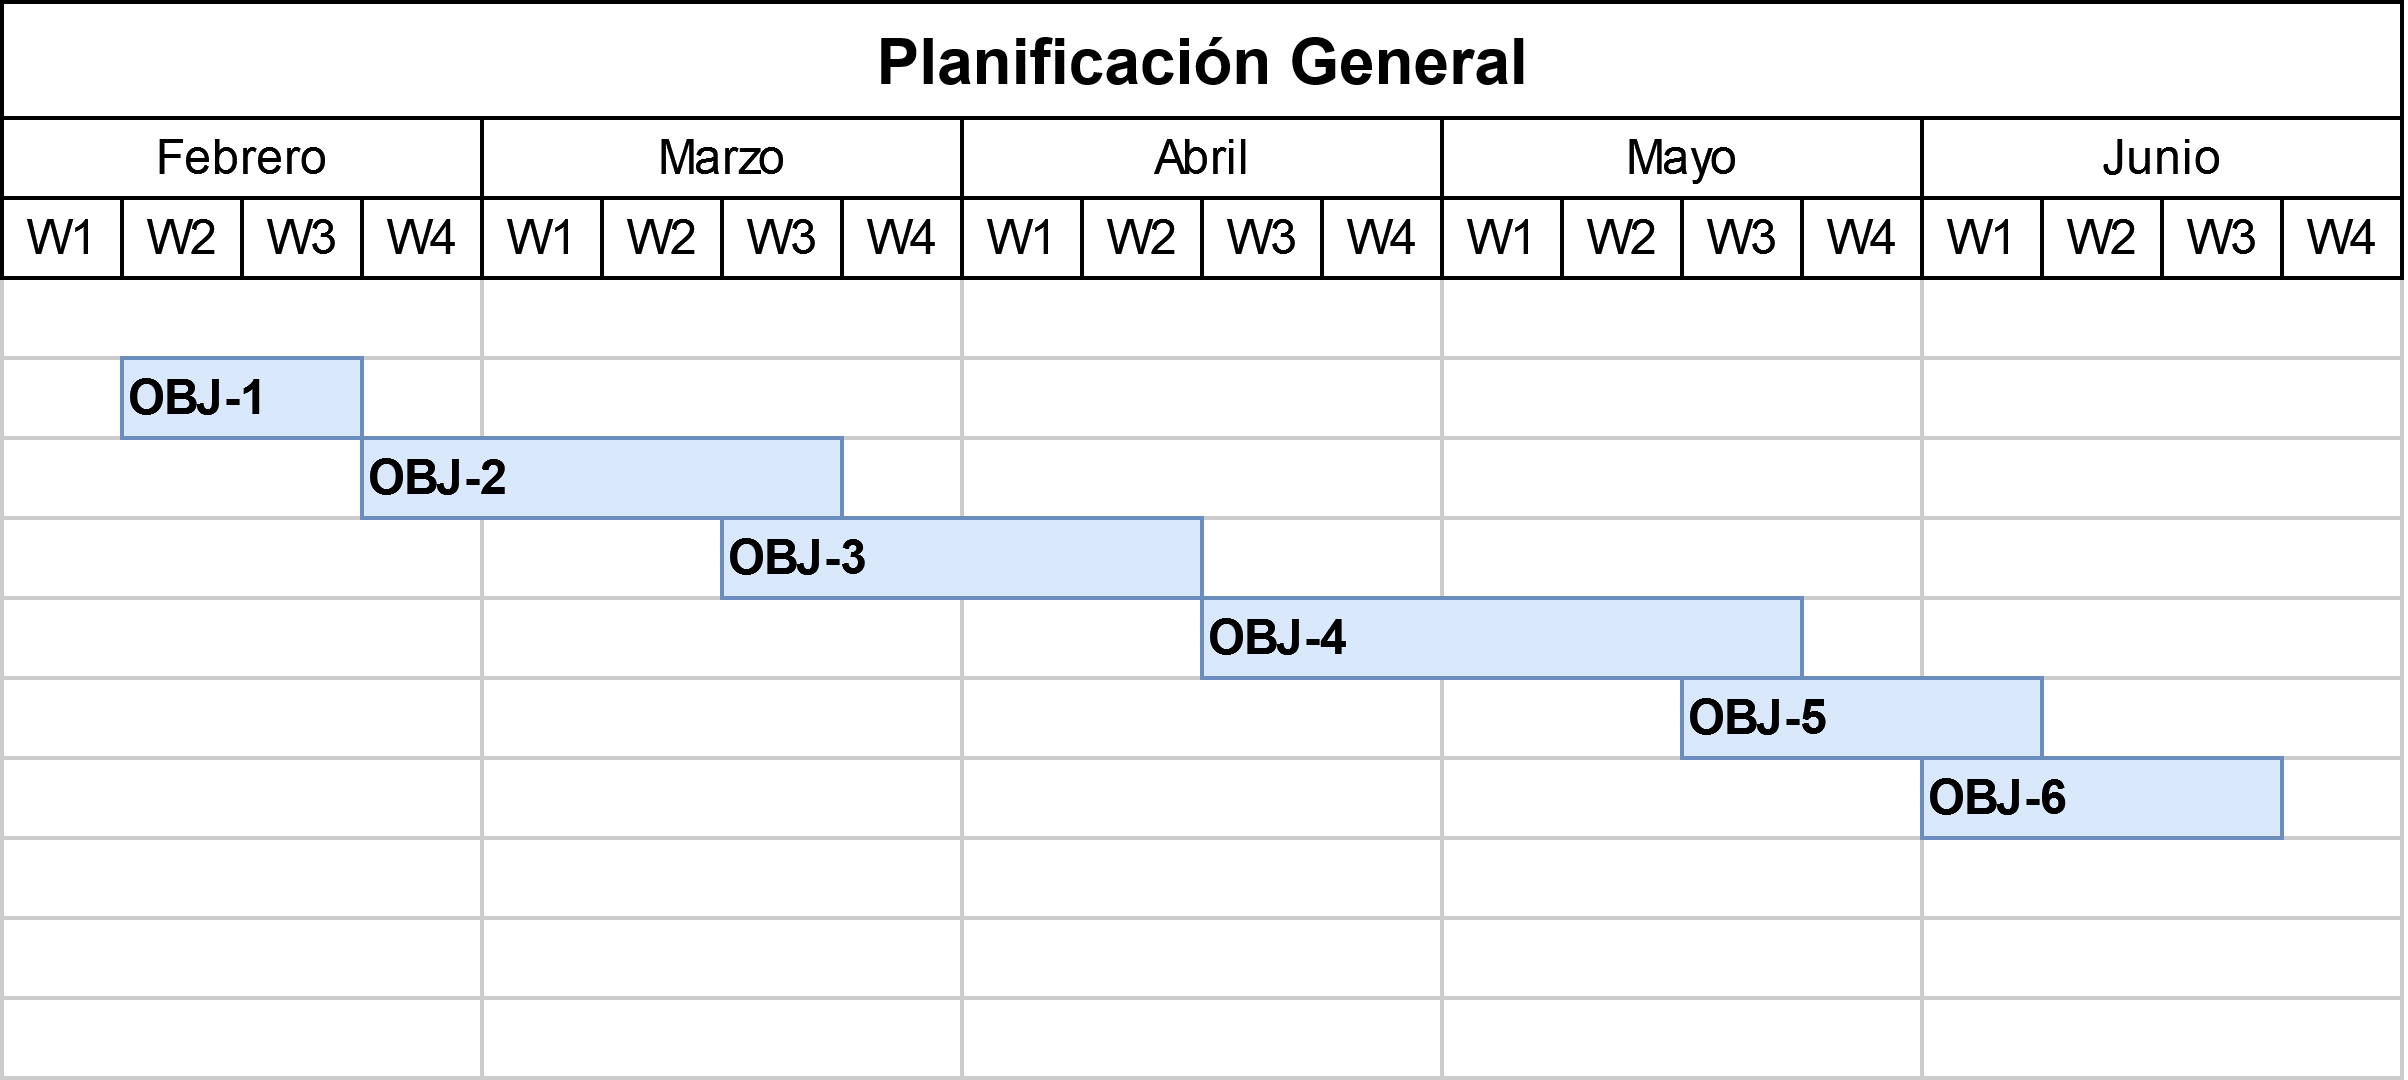
\includegraphics[width=0.99\textwidth]{img/fig/fig1.4-gantt.png}
    \caption{Planificación de este trabajo}
    \label{fig:gantt}
\end{figure}

Por supuesto, esta planificación es aproximada y flexible hasta cierto punto.
Debido a la naturaleza de este trabajo, es difícil preveer con exactitud el correcto desarrollo de la planificación,
al requerir un estudio constante de una tecnología en desarrollo con multitud de opciones, así como la dependencia de un proyecto de ámbito \textit{open source},
en constante evolución con los posibles problemas y contratiempos que ello puede ocasionar, por ejemplo, las actualizaciones de este.

En el último capítulo, se hará una comparación entre esta planificación y el resultado final de esta, 
con objetivo de entender que ha pasado durante el desarrollo de este trabajo
y si el desarrollo ha ido como fue planeado. 